% !TEX root = rapport_root.tex
\subsection{Fine-tuned SciBERT LLM}
\subsubsection{Implementation}
To evaluate the effectiveness of transformer-based language models for scientific section classification, we fine-tune SciBERT on a subset of our dataset. To construct a high-confidence training/testing dataset, sections were grouped based on title (see \cref{tab:101}), resulting in subset of 2046 samples spread equally over 6 separate classes.
\begin{table}[h!]
\centering
\begin{tabular}{|c|l|}
\hline
\textbf{Label ID} & \textbf{Section Titles (Canonical Variants)} \\
\hline
0 & INTRODUCTION \\
\hline
1 & METHODS, METHODOLOGY, METHOD \\
\hline
2 & DATA AND RESULTS, RESULTS, FINDINGS \\
\hline
3 & DISCUSSION, DISCUSSION AND CONCLUSIONS \\
\hline
4 & CONCLUDING REMARKS, CONCLUSION, CONCLUSIONS \\
\hline
5 & THEORY, BACKGROUND, THEORETICAL FRAMEWORK, \\
  & THEORETICAL BACKGROUND, LITERATURE REVIEW \\
\hline
\end{tabular}
\caption{Canonical section title groups used for high-confidence label assignment.}
\label{tab:101}
\end{table}

Fine-tuning was implemented with the Huggingface Transformers library, initializing the model using the 'allenai/scibert\_scivocab\_uncased' checkpoint and 'AutoModelForSequenceClassification' class. Tokenization was handled using the corresponding 'AutoTokenizer', truncated to a maximum of 512 tokens and padded to ensure homogeneous data length. Since we are only doing transfer learning, the embedding and encoder model layers were frozen, relying on iterative adjustment of the final pooler layers to aggregate model output into an interpretable classification output vector. The final model was optimized using a 30-35-35 training-testing-validation-split to minimize overfitting, with hyperparameters
$$
l_r = 2\cdot 10^{-4}, \quad \text{Batch Size} = 8, \quad \text{Epochs} = 10.
$$
(see notebook 'bert\_section\_classifier.ipynb' for full implementation)
\subsubsection{Results and Discussion}
The model was trained locally on an NVIDIA GPU over the span of $\sim$7 hours. Key training and evaluation metrics (summarized in \cref{tab:102}) show a steady decrease in training and evaluation loss from 1.3488 and 1.0107 after the first epoch to 0.5358 and 0.5754 after epoch 10, respectively. Model accuracy on evaluation data showed a corresponding increase from 0.638 to 0.769 during the same period, suggesting that the model is learning generalizable patterns rather than overfitting to the data. Notably, the metrics also show a clear plateau around epoch 7-8, suggesting that further mode convergence does not result in any noticable performance improvements. Reducing training to 8 epochs may therefore save time and computational resources without adversely affecting model classification capabilities.

\begin{table}[h!]
\centering
\begin{tabular}{|c|c|c|c|c|c|}
\hline
\textbf{Epoch} & \textbf{Train Loss} & \textbf{Eval Loss} & \textbf{Eval Accuracy} & \textbf{Learning Rate} & \textbf{Grad Norm} \\
\hline
1  & 1.3488 & 1.0107 & 0.638 & 1.80e-4 & 5.63 \\
2  & 0.9062 & 0.8415 & 0.668 & 1.60e-4 & 5.11 \\
3  & 0.7612 & 0.7020 & 0.717 & 1.40e-4 & 4.19 \\
4  & 0.6701 & 0.6754 & 0.746 & 1.20e-4 & 6.02 \\
5  & 0.6338 & 0.6465 & 0.749 & 1.00e-4 & 3.16 \\
6  & 0.6026 & 0.6249 & 0.752 & 8.01e-5 & 3.58 \\
7  & 0.5862 & 0.6030 & 0.772 & 6.01e-5 & 3.16 \\
8  & 0.5716 & 0.5855 & 0.772 & 4.01e-5 & 3.72 \\
9  & 0.5560 & 0.5835 & 0.765 & 2.01e-5 & 3.34 \\
10 & 0.5358 & 0.5754 & 0.769 & 1.12e-7 & 5.54 \\
\hline
\end{tabular}
\caption{Training and evaluation metrics for SciBERT across 10 epochs.}
\label{tab:102}
\end{table}

\Cref{tab:103} presents model evaluation on validation data. Overall accuracy was found to be 0.772. The precision and recall of 0.791 and 0.772, respectively, and the resulting F1-score of 0.776, indicate balanced false-positive and false-negative across the classes. The log loss of 0.646 suggests relatively high model confidence when making correct choices and large uncertainty when making incorrect ones. This is further reinforced by an average confidence of 0.750 and average entropy of 0.645, implying (generally) sharply focused model prediction with low uncertainty and diffuseness. Examining \Cref{tab:104} and \Cref{fig:101} reveals average model performance on sections "Introduction", "Conclusion" and "Discussion", with higher predictive ability on sections "Methods" and "Results" and a rather lackluster F1-score of 0.629 on "Theory" sections. \Cref{fig:101} indicates that this performance drop is a concequence of frequent misclassification of "Theory" sections as "Introduction", and vice versa. Interestingly, the matrix shows elevated numbers for diagonal-adjacent tiles, suggesting that false label assignments primarily occur between "bordering" article sections. This hints at the fact that articles trace a continuous "semantic path" from beginning to end, resulting in textually adjacent sections being more closely related (and therefore harder to distinguish). We will explore this characteristic more thoroughly in later analysis.

\begin{table}[ht]
\centering
\caption{Overall Evaluation Metrics on Validation Data}
\begin{tabular}{lcc}
\toprule
\textbf{Metric} & \textbf{Value} \\
\midrule
Accuracy               & 0.772 \\
Precision   & 0.791 \\
Recall      & 0.772 \\
F1-score    & 0.776 \\
Log Loss               & 0.646 \\
Average Confidence     & 0.750 \\
Average Entropy        & 0.645 \\
\bottomrule
\end{tabular}
\label{tab:103}
\end{table}

\begin{table}[ht]
\centering
\caption{Per-Class Evaluation Metrics}
\begin{tabular}{lcccc}
\toprule
\textbf{Class} & \textbf{Precision} & \textbf{Recall} & \textbf{F1-score} & \textbf{Support} \\
\midrule
Introduction          & 0.759 & 0.721 & 0.739 & 61 \\
Theory                & 0.550 & 0.733 & 0.629 & 45 \\
Methods               & 0.933 & 0.808 & 0.866 & 52 \\
Results               & 0.785 & 0.911 & 0.843 & 56 \\
Discussion            & 0.809 & 0.731 & 0.768 & 52 \\
Conclusion            & 0.906 & 0.707 & 0.795 & 41 \\
\bottomrule
\end{tabular}
\label{tab:104}
\end{table}

\begin{figure}%[h!]
    \centering
    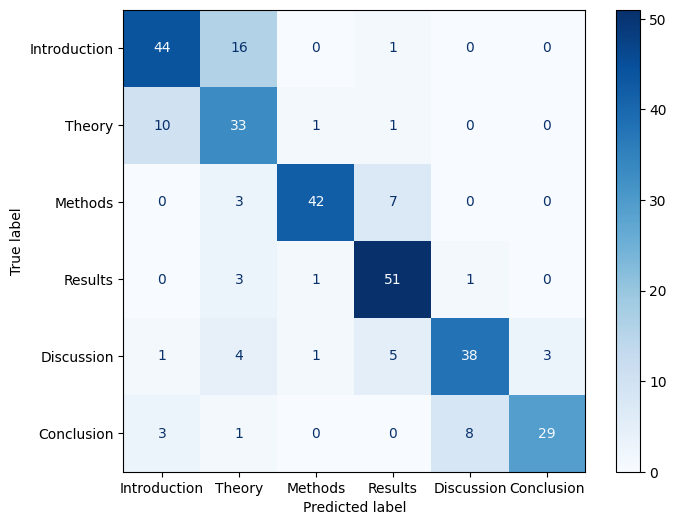
\includegraphics[width=.6\linewidth]{media/transformer_confusion_matrix.png}
    \caption{Confusion Matrix outlining model performance on validation split.}
    \label{fig:101}
\end{figure}

\subsection{Projection Based Classification}
While fine-tuning a language model is effective, it is often computationally demanding, time-consumimg, and unecessary complex for simple og low-resource applications. Leveraging the geometric properties of textual embeddings, we iteratively develop and implement a lightweight classification approach that offers a fast, interpretable and data-efficient alternative to full fine-tuning. To maintain alignment with prior benchmarks, we rely on the same six-category classification dataset as used in SciBERT fine-tuning. All data are encoded using the text-embedding-3-large model from OpenAI.

\subsubsection{Implementation}
\paragraph{Mean Embedding Similarity}
Given a small number of labeled samples per class, we calculate class wise means represent the prototypical embedding of each class in the semantic space. These mean vectors serve as centroids, or "semantic signatures", and summarize the contextualized representations of each class. The similarity of a given sample $x$ to a given class is calculated using the inner product
\begin{equation}
    \text{sim}(x, \mu_{c}) = \braket{x, \mu_c}
\end{equation}
where $\mu_c$ is the respective, normalized, class mean. The resulting score can be interpreted as a measure of sample-class alignment. Returning to the data-subset used for fine-tuning previously, we create a new dataframe containing only instances of "Introduction" and "Results" (arbitrarily chosen). Calculating an "Introduction" mean, we associate a score with each sample using (1). Sorting the data by this score, we see a clear class seperation (see \cref{fig:102} (2)).

\begin{figure}%[H]
    \centering
    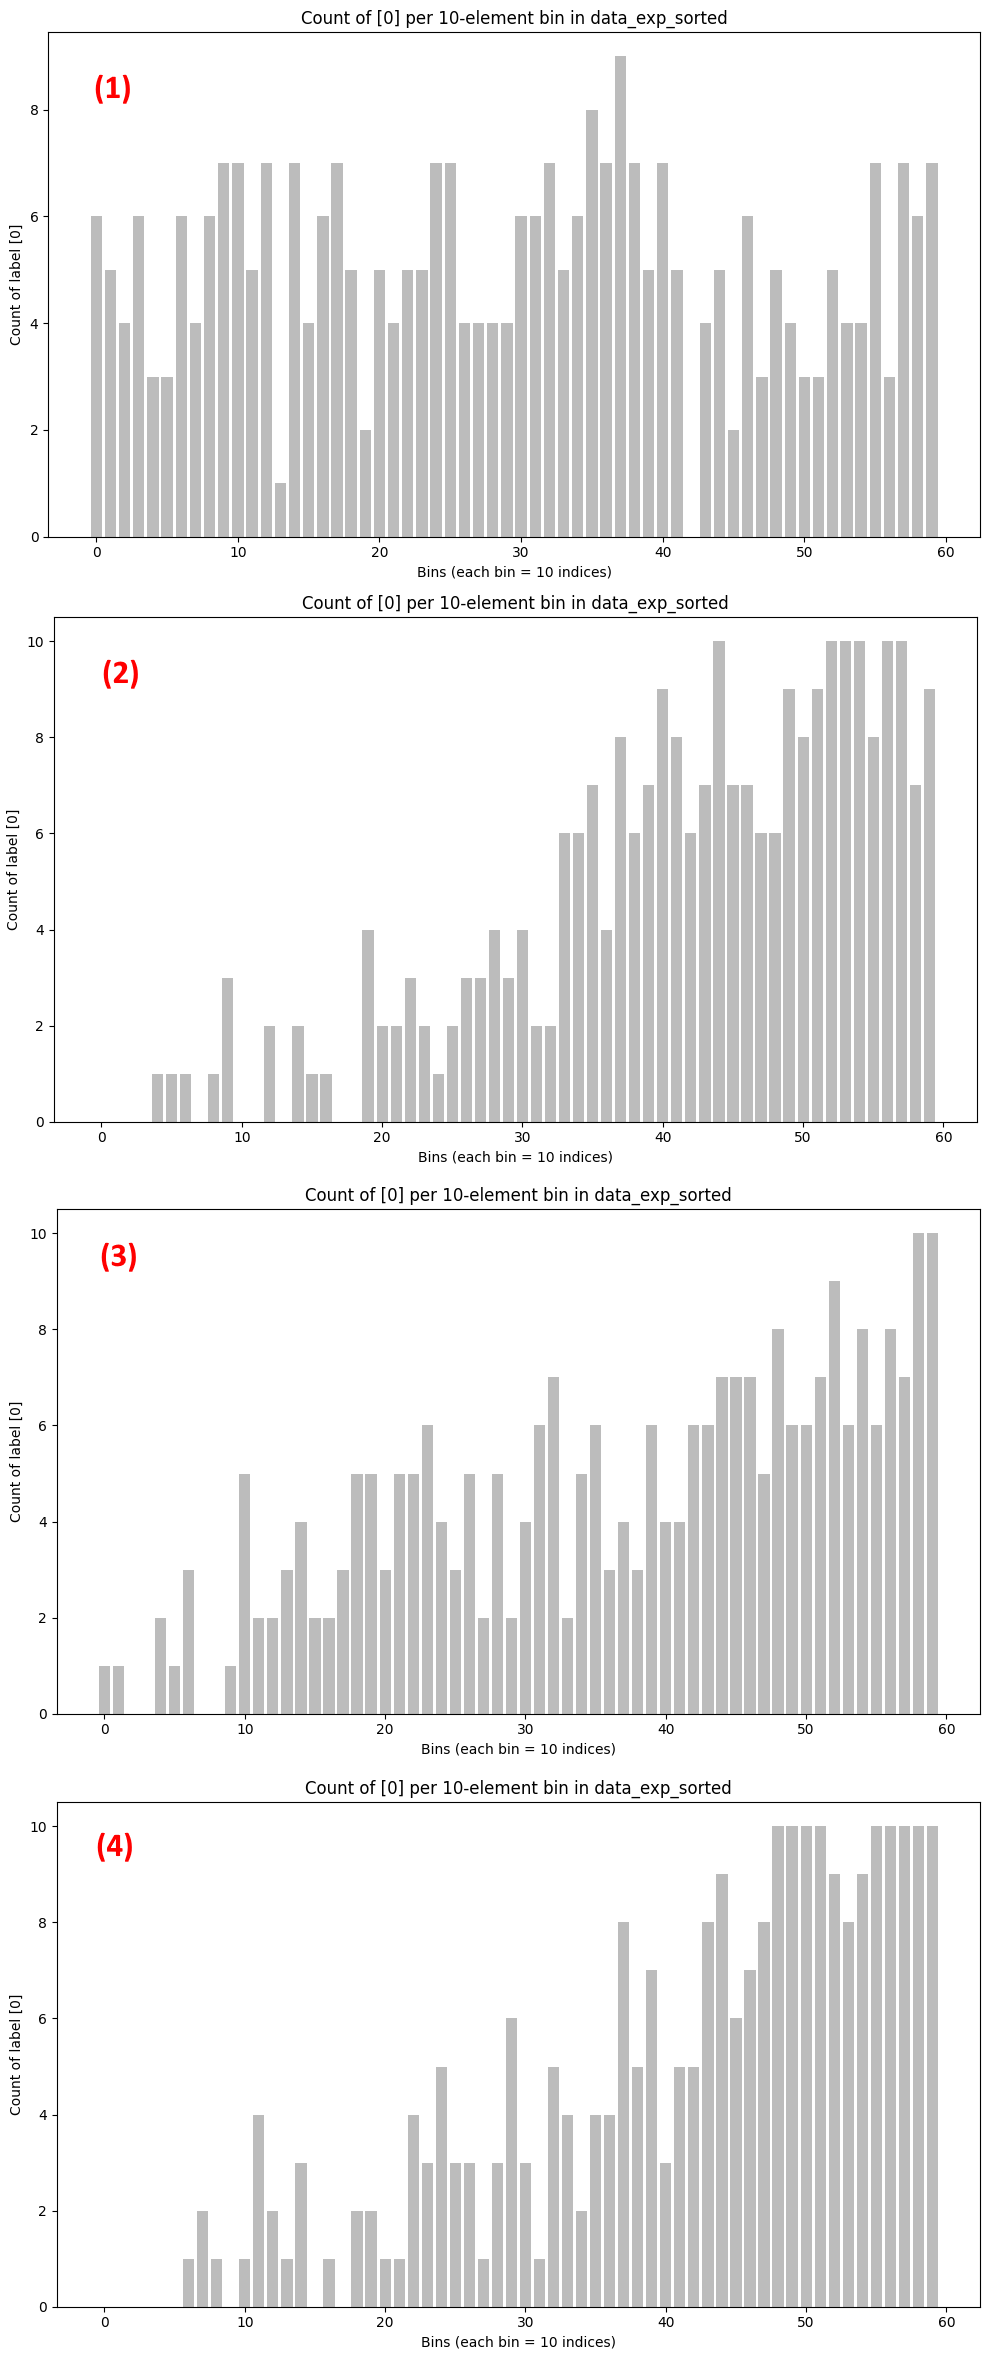
\includegraphics[width=0.5\linewidth]{media/score_sorting.png}
    \caption{Distribution of labels in dataset. A bin along the x-direction represent a 10 consecutive data entries, with the number along the y-axis indicating percentage of label 0 among the entries.}
    \label{fig:102}
\end{figure}

\paragraph{Class-centroid Difference Scoring}
Given last paragraphs inerpretation of class centroids as being prototypical representation of each class, it seems intuitive that the difference vector $v = \mu_2-\mu_1$ between two class centroids $\mu_{1}$ and $\mu_{2}$ should somehow "encode" the semantic difference between the classes. In other words, $v$ captures how the meaning of class 1 diverges from that of class 2 in the embedding space. It might therefore also be interesting to get a measure of where a sample embedding falls along this seperation axis. For any sample $x$, we take its projection onto the centroid difference vector (see \cref{fig:103})
\begin{equation}
    \text{proj}_{v}(x) = \frac{\braket{x, v}}{\braket{v, v}}v = \braket{x, v}v = k\cdot v, \quad k = \braket{x, v}
\end{equation}
where we assume that the difference vector $v$ has already been normalized $|v| = 1$. In the end result $v$ is independent of $x$, and we are left with the inner product $k$ being the metric of interest, indicating the position of a sample projection along the seperation axis, ranging from $k = -\infty$ (really far in direction of Class 1) to $k = \infty$ (really far in direction of Class 2).
\begin{figure}%[h]
    \centering
    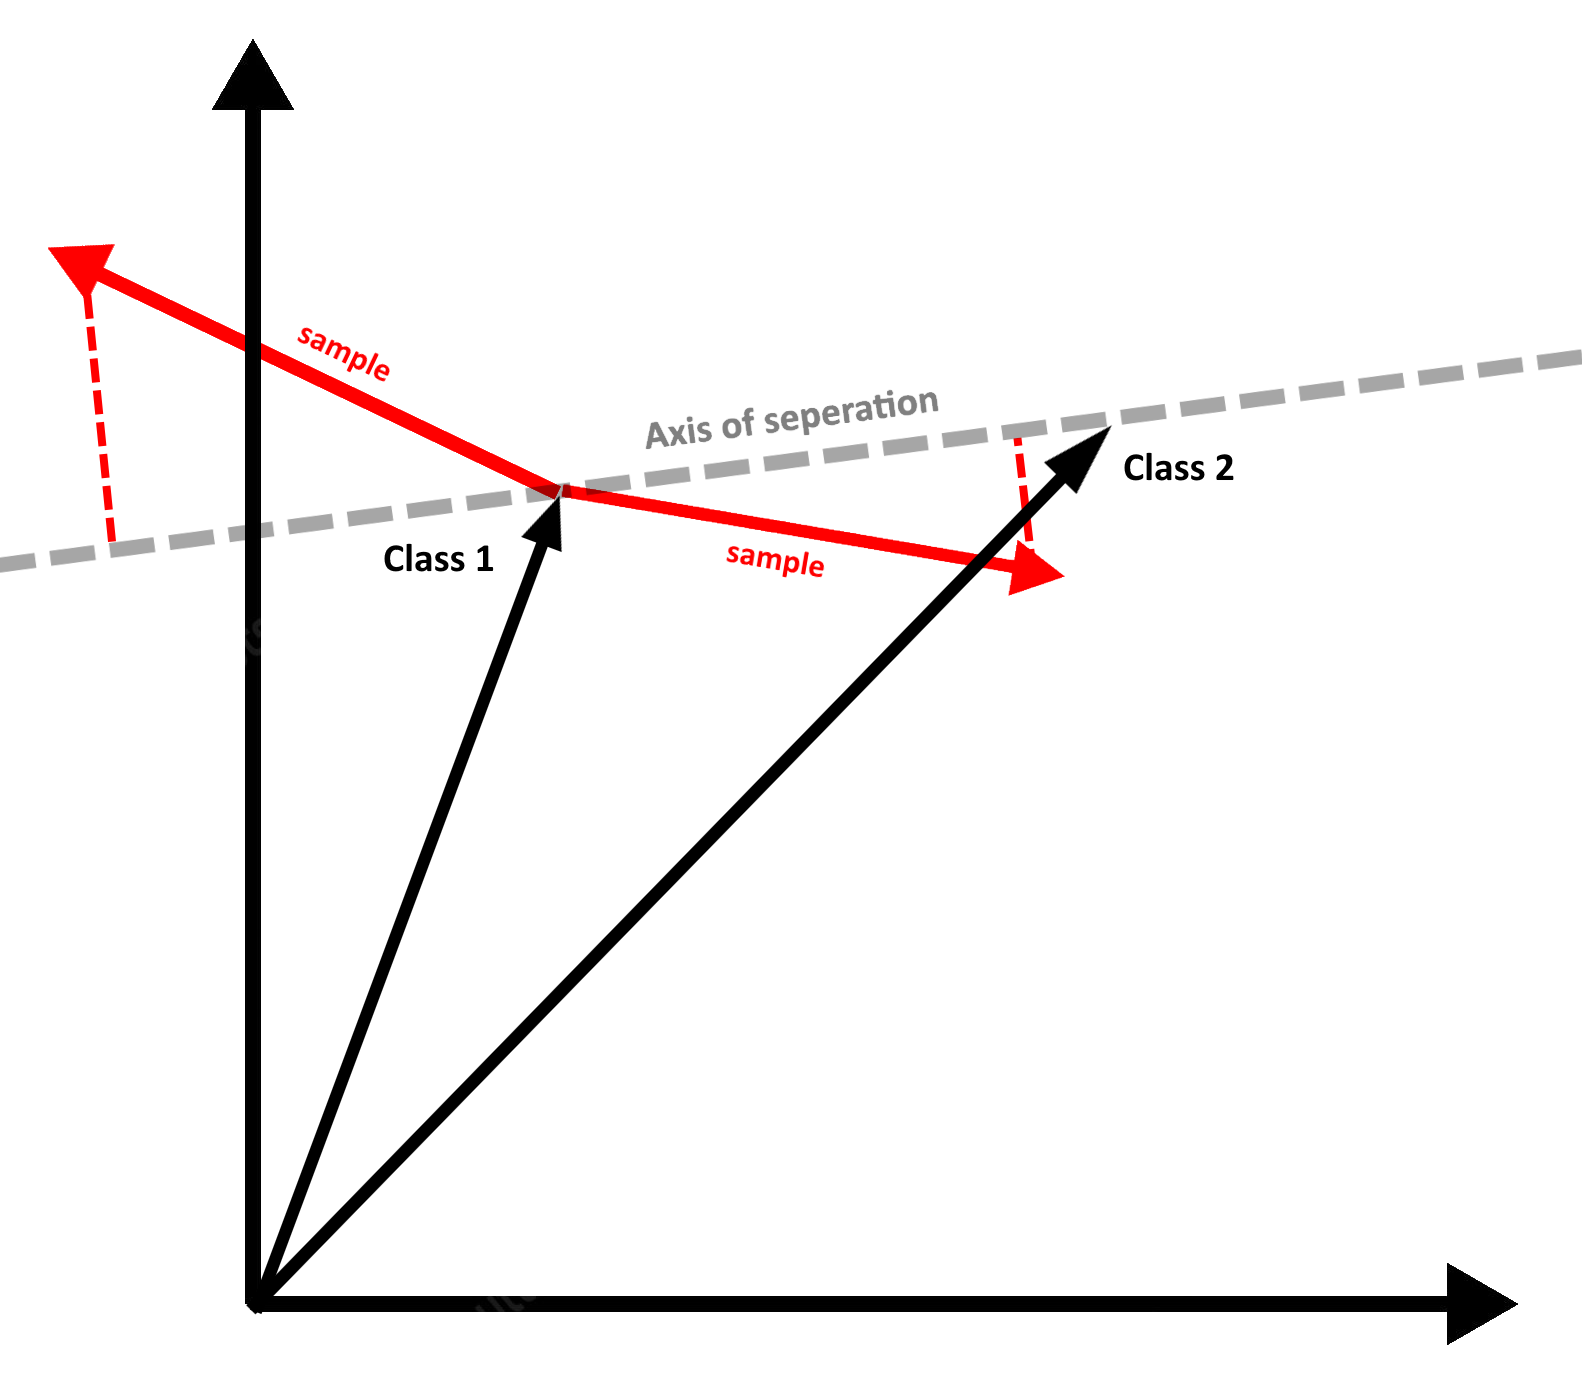
\includegraphics[width=0.5\linewidth]{media/vec_diff_graphic.png}
    \caption{Geometric visualization of the centroid difference vector and the projection upon it.}
    \label{fig:103}
\end{figure}
In the end we are left with a "seperation" score
\begin{equation}
    \text{sep}(x, v =\mu_{c2}-\mu_{c1}) = \braket{x, v}
\end{equation}
Testing again on the aforementioned "Introduction/Results" dataset, we calculate a centroid difference vector and associate a "seperation" score with each sample. Sorting the data by this score, we again see a clear class seperation (see \cref{fig:102} (3)).
\paragraph{Combined Scores and Binary Model Implementation}

These scores are in a sense complementary, with "similarity" scores measuring sample alignment with centroids and "seperation" scores measuring sample-centroid displacement. Combining the two into a single, combined, score
\begin{equation}
    \text{score} = \lambda \cdot \text{sim}(x, \mu_{c1})+(1-\lambda)\cdot \text{sep}(x, \mu_{c2}-\mu_{c1})
\end{equation}
where score weighting is adjusted by varying $\lambda$. Arbitrarily choosing $\lambda = 0.5$ and sorting the same data as before by this new score, we seemingly obtain the best class separation yet (\Cref{fig:102} (4)). Using this combined score, we implement a binary classification model and test it on all $\begin{pmatrix}
    6\\
    2
\end{pmatrix}$ binary 6-class combinations (still testing on the same 2046-sample dataset used previously) using a 0.7/0.3 train-test-split. The decision threshold for assigning binary labels is defined as the median of the score distribution. We also evaluate model performance on the training split for a range of $\lambda\in[0, 1]$ to find optimal score-weighting.

\begin{table}[ht]
\centering
\caption{Summary of Binary Classification Metrics Across All Class Pairs}
\begin{tabular}{lcccc}
\toprule
\textbf{Statistic} & \textbf{Accuracy} & \textbf{Precision} & \textbf{Recall} & \textbf{F1-score} \\
\midrule
\textbf{Mean}   & 0.902             & 0.904              & 0.900           & 0.901 \\
\textbf{Maximum}   & 0.976             & 0.989              & 0.990           & 0.974 \\
\textbf{Minimum}   & 0.732             & 0.755              & 0.705           & 0.729 \\
\bottomrule
\end{tabular}
\label{tab:105}
\end{table}

\noindent \Cref{tab:105} shows a generally strong and balanced model performance above 0.900 across the board, with maximum performance in the high 0.900s. Introduction/Theory classification is however an outlier, with values in the low 0.700s. This comes as no suprise given our previous findings with the fine-tuned SciBERT model.


(see notebook "nonMLP\_classifier.ipynb" for full implementation)
\subsubsection{Full Multi-Class Classification Model}

\paragraph{Non-MLP Implementation}

Multi-class classification ability is handled using a One-vs-One (OvO) approach, which involves fitting a distinct binary classifier to all $\begin{pmatrix}
    n_{\text{classes}}\\
    2
\end{pmatrix}$ class combinations. Each binary classifier in the ensemble operates using the lightweight scoring approach outlined above, calculating class means, combined scores according to (4), with individually optimized $\lambda$-weighting. When applied to a sample, each constituent classifier casts a binary vote, and final model prediction is aggregated using a majority vote. The model was fitted to the data, taking sub-5 seconds. It was then evaluated on the test split using key metrics, presented in \Cref{tab:106}, \Cref{tab:107} and \Cref{fig:104}.

\begin{table}%[ht]
\centering
\caption{Overall Evaluation Metrics for Non-MLP Classifier}
\begin{tabular}{lr}
\toprule
\textbf{Metric} & \textbf{Value} \\
\midrule
Accuracy            & 0.713 \\
Precision & 0.715 \\
Recall    & 0.713 \\
F1-score  & 0.713 \\
Log Loss             & 1.275 \\
Average Confidence   & 0.331 \\
Average Entropy      & 1.494 \\
\bottomrule
\end{tabular}
\label{tab:106}
\end{table}

\begin{table}%[ht]
\centering
\caption{Per-Class Evaluation Metrics}
\begin{tabular}{lcccc}
\toprule
\textbf{Class} & \textbf{Precision} & \textbf{Recall} & \textbf{F1-score} & \textbf{Support} \\
\midrule
Introduction      & 0.568 & 0.636 & 0.600 & 118 \\
Methods           & 0.867 & 0.875 & 0.871 & 104 \\
Results           & 0.787 & 0.842 & 0.813 & 101 \\
Discussion        & 0.646 & 0.634 & 0.640 & 101 \\
Conclusion        & 0.767 & 0.702 & 0.733 & 94  \\
Theory            & 0.679 & 0.594 & 0.633 & 96  \\
\bottomrule
\end{tabular}
\label{tab:107}
\end{table}

\begin{figure}%[ht]
    \centering
    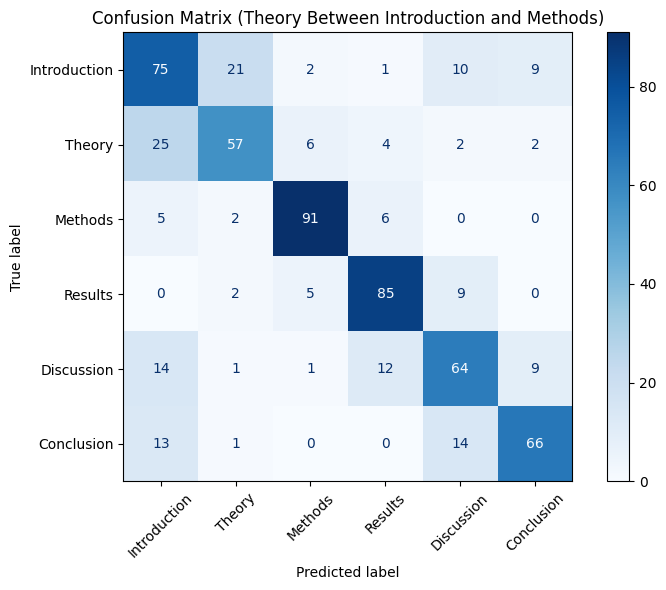
\includegraphics[width=0.6\linewidth]{media/nonML_confusion_matrix.png}
    \caption{Confusion Matrix outlining non-MLP model performance on test split.}
    \label{fig:104}
\end{figure}
\noindent (see notebook 'nonMLP\_classifier.ipynb' for full implementation)
\paragraph{MLP Implementation}
To further enhance model performance, we replace the majority voting system with a multi-layer perceptron (MLP), trained to map the combined projection scores to class logits. Using the same OvO-approach, the resulting scores are fed into an MLP with input dimensions $2\cdot \begin{pmatrix}
    n_{\text{classes}}\\
    2
\end{pmatrix}$. That is, weighting using the aforementioned $\lambda$ is discarded in favour of directly inputting all scores into the neural network. The input layer is succeeded by three ReLU-activated hidden layers, gradually consolidating the input into fewer dimensions, resulting finally in an output layer producing a single logit for each class.

%\Testing % @Lars, what is this?
for a range of different hyperparameters (see notebook 'mlp\_classifier.ipynb' for more details), optimal performance on the data was found for the following parameters
$$l_r = 5\cdot 10^{-4}, \quad \text{Hidden Layer Dimensions} = [32, 16, 8], \quad \text{Epochs} = 200.$$

Model fitting completed in under 10 seconds. Resulting model performance is outlined in \Cref{tab:108}, \Cref{tab:109}, \Cref{tab:110} and \Cref{fig:105}.

\begin{figure}%[ht]
    \centering
    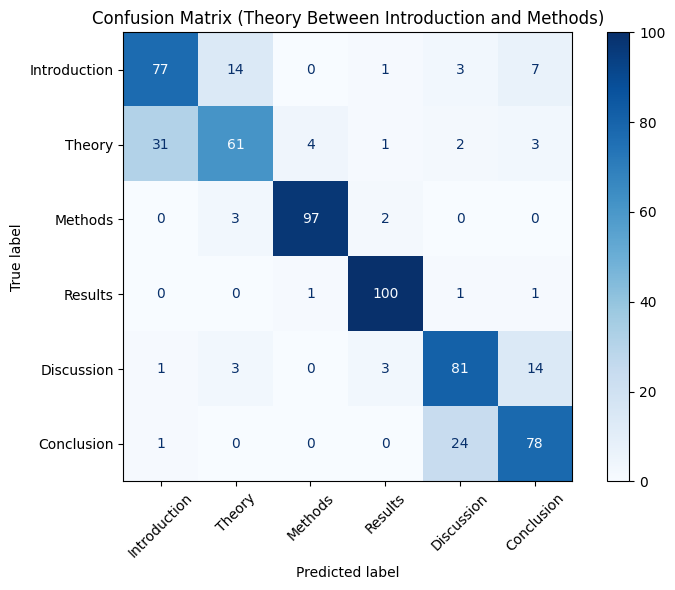
\includegraphics[width=0.6\linewidth]{media/MLP_confusion_matrix.png}
    \caption{Confusion Matrix outlining MLP model performance on test split.}
    \label{fig:105}
\end{figure}
\begin{table}[ht]
\centering
\caption{Summary of Binary Classification Metrics}
\begin{tabular}{lcccc}
\toprule
\textbf{Statistic} & \textbf{Accuracy} & \textbf{Precision} & \textbf{Recall} & \textbf{F1-score} \\
\midrule
Average & 0.902 & 0.903 & 0.905 & 0.903 \\
Maximum & 0.985 & 0.991 & 1.000 & 0.986 \\
Minimum & 0.751 & 0.737 & 0.771 & 0.767 \\
\bottomrule
\end{tabular}
\label{tab:108}
\end{table}

\begin{table}[ht]
\centering
\caption{Overall Evaluation Metrics for MLP Classifier}
\begin{tabular}{lc}
\toprule
\textbf{Metric} & \textbf{Value} \\
\midrule
Accuracy               & 0.805 \\
Precision   & 0.804 \\
Recall     & 0.805 \\
F1-score    & 0.803 \\
Log Loss               & 0.529 \\
Average Confidence     & 0.786 \\
Average Entropy        & 0.552 \\
\bottomrule
\end{tabular}
\label{tab:109}
\end{table}

\begin{table}[ht]
\centering
\caption{Per-Class Evaluation Metrics for MLP Classifier}
\begin{tabular}{lcccc}
\toprule
\textbf{Class} & \textbf{Precision} & \textbf{Recall} & \textbf{F1-score} & \textbf{Support} \\
\midrule
Introduction & 0.700 & 0.755 & 0.726 & 102 \\
Theory & 0.753 & 0.598 & 0.667 & 102 \\
Methods & 0.951 & 0.951 & 0.951 & 102 \\
Results & 0.935 & 0.971 & 0.952 & 103 \\
Discussion & 0.730 & 0.794 & 0.761 & 102 \\
Conclusion & 0.757 & 0.757 & 0.757 & 103 \\
\bottomrule
\end{tabular}
\label{tab:110}
\end{table}


\subsubsection{Model Comparison and Discussion}
The projection classification model offer a lightweight alternative to full fine-tuning. From \Cref{tab:105}, \Cref{tab:106} and \Cref{tab:107} we see that the non-MLP variant performs well on binary classification tasks (both accuracy and F1 score above 0.9), but multi-class classification performance is significantly worse (accuracy and F1-score of 0.713) class wise performance even lower (F1-score of 0.600) on "Introduction" sections. Looking at \Cref{fig:104} it is evident that the model suffers from the same diagonal-adjacent class mislabeling, but in addition it also frequently misclassifies "Introductions" as "Discussion/Conclusion" and vice versa. The implementation also suffers from a large flaw; the decision threshold from label assignment is based on the median of the score distribution. This results in a model that is extreme sensitive to class imbalances in the training split. To examine this we test binary classification performance on "Introduction" and "Methods" sections for differing label imbalances. A 1:1 label relation results in a classification performance of $\sim$0.95. This number decreases to $\sim$0.84 for a label imbalance of 2:1, and increasing the discrepancy to 4:1 results in a performance drop to $\sim$0.73.


The MLP-approach replaces this fixed threshold strategy with a trainable component capable of learning non-linear relationships between class score-pairs. \Cref{tab:108} shows that this does not seem to increase binary classification performance, with very little improvement in mean (though minimum performance does increase from an F1-score 0.729 to 0.767). Comparing \Cref{tab:106} and \Cref{tab:109} shows significant improvements in multi-class performance, with accuracy and F1-scores increasing from 0.713 and 0.713 to 0.805 and 0.803, respectively. Average model confidence also increase by almost 2.5x, while average entropy is cut by 2/3 the original value (though these gains do come at the cost of intuitiveness/interpretability). Looking at \Cref{fig:105} we see that misclassifications are now limited almost completely to "Introduction/Theory" and "Discussion/Conclusion". We also tried to train several MLPs in parallel, mimicking a sort of weak learning approach, with final output being the mean of all estimators. Testing for $n_{\text{estimators}}\in [1, 2, 4, 8, 16]$ over a range of hyperparameters, we saw very-slight to nonexistent performance improvements ($\sim 1\%$) on our data, indicating that this does not yield any significant advantage.


Comparing these projection models with the fine-tuned SciBERT model we see that the MLP-variant outperforms the fine-tuned LLM, with higher accuracy (0.805 v. 0.772), F1-score (0.803 v. 0.776), higher confidence (0.786 v.0.750) and lower entropy (0.552 v. 0.645). While not as fast as the non-MLP model (sub 5-second training time), the MLP model delivers performance rivaling the fine-tuned LLM at a fraction of the computational cost and time (sub 10-second v. $\sim$7hrs). It is also more data-efficient (though the MLP-variant is less so), primarily utilizing few shot sampling of 8 examples per class. \Cref{fig:106} shows that the means calculated using $n$ samples converges to the global mean using all samples very quickly, suggesting that sampling only a few examples does not significantly impact performance. Testing on the models reflects this fact; increasing the number pof samples $n$ results only in very slight performance gains ($\sim$1\%) on our data. This indicates that these projection models are a lightweight alternative to full-on model fine-tuning, offering competitive performance with greatly improved computational- and data efficiency.

\begin{figure}%[h!]
    \centering
    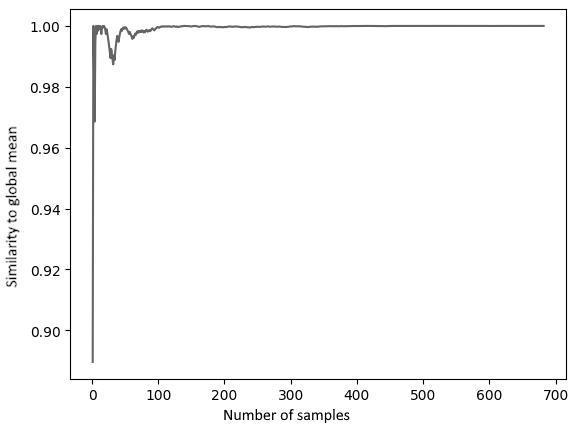
\includegraphics[width=0.7\linewidth]{media/few_shot_sampling.png}
    \caption{Inner product of normalized average of $n$ embeddings with global average. We see that it quickly approaches 1.}
    \label{fig:106}
\end{figure}


While these projection models do not utilize computationally intensive transformers, they depend on the existence of high quality embedding models. In fact, the models are very sensitive to the quality of the embeddings. The data, instead embedded using the 'Voyager-3-large' embedding model, immediately causes a sharp performance drop of $\sim 7\%$ (relative). This approach is lightweight and quick only if embeddings are precomputed; in other words, it is still implicitly dependent on large, compute- and data hungry models, leading the real computational cost to be much higher than these results give the impression of. This juxtaposition risks completely invalidating the model’s original motivation and conceptual justification. It also raises another important point; while the projection models utilize cutting-edge, modern embedding models, the SciBERT implementation uses its own aging tokenizer, perhaps resulting in lower quality input and thereby rendering the comparison between the two unfair and biased.

\subsubsection{2D visualization of score-pairs}
Visualizing these score pairs seems an interesting prospect, perhaps yielding some new insight or intuition. Returning to the same dataset as earlier, we calculate the global mean embedding and the difference vector between the "Introduction"- and "Conclusion" mean centroids. Finding the aforementioned "similarity" and "seperation" scores of all section samples and plotting them as 2-dimensional points (\Cref{fig:107}), we see clear clustering on a section-type basis. What is perhaps most interesting is how this contrasts with earlier findings; using other dimensional-reduction techniques, sections seemed to display thematically based clustering. This plot seems to indicate the opposite (perhaps this is caused by the fact that the specially selected "Introduction/Conclusion" difference vector specifically "picks out" the sample-embedding characteristics most similar to its own?). Instead plotting the means of $\sim$20 embeddings on a class by class basis (attempting to reduce semantic noice), we see a clear seperation of classes (see \Cref{fig:108}). 

\begin{figure}%[H]
    \centering
    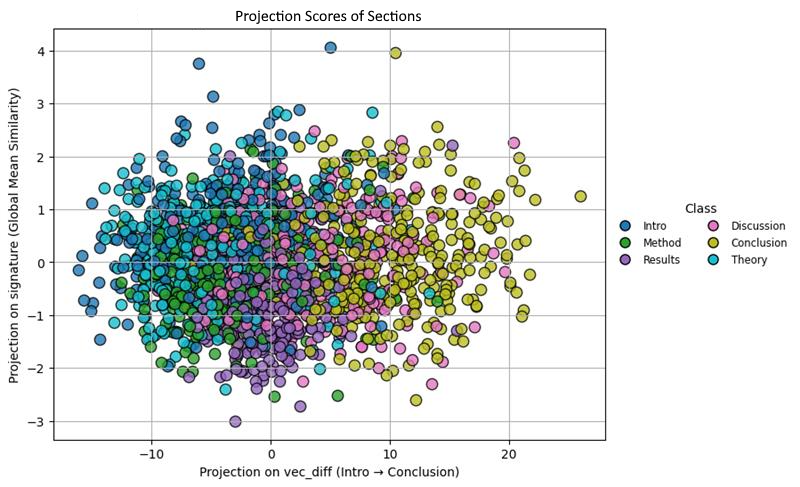
\includegraphics[width=.8\linewidth]{media/section_projections.png}
    \caption{2D projection scores of sections onto Introduction/Conclusion difference vector (x-axis) and global average embedding (y-axis).}
    \label{fig:107}
\end{figure}


Interestingly, the clusters trace out the semantically logical path from "Introduction" to "Conclusion" along the x-axis, indicating that the "Intro/Conclusion" difference vector seemingly captures the entire semantic path of the article from beginning to end, with "Introduction" and "Conclusion" at each side, "Theory" and "Methods" very similar to "Introduction", and "Results" and "Discussion" progressively moving towards the right. The y-axis also shows "Introductions" as being the most similar to the global mean and "Results" as being the most divergent. Furthermore, the proximity of "Introduction" and "Theory" reinforces the earlier result that the sections-classes are closely related, given that they were often mistakenly interchanged by the classification models.

\begin{figure}%[h!]
    \centering
    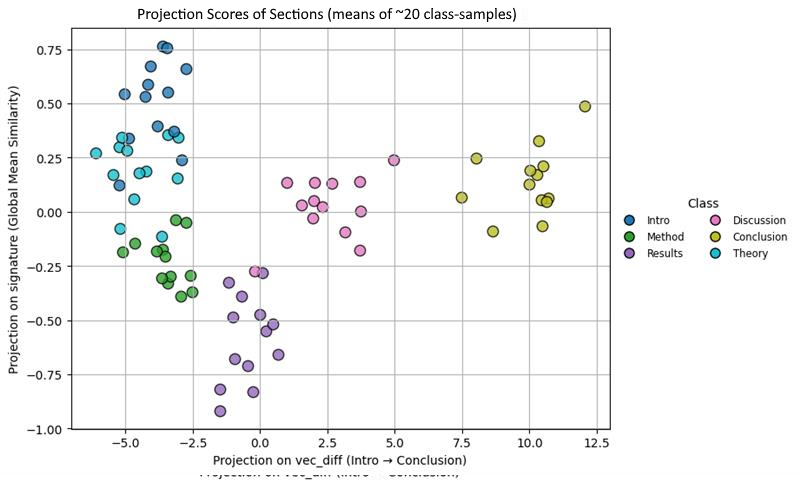
\includegraphics[width=.8\linewidth]{media/mean_section_projections.png}
    \caption{2D projection scores of mean embeddings of ~20 sections of same type onto Introduction/Conclusion difference vector (x-axis) and global average embedding (y-axis).}
    \label{fig:108}
\end{figure}

This visualization tool provides a different way of considering the projection scores, and will be used extensively during further analysis.